\begin{frame}[shrink=20]
  \frametitle{Agenda}
  \begin{itemize}
    \item Introducción:
      \begin{itemize}
        \item Aplicaciones web y la seguridad.
        \item Mecanismos de protección.
        \item ¿Qué es un WAF?
      \end{itemize}
    \item Situación actual. Estado del arte:
      \begin{itemize}
        \item Soluciones WAF privativas.
        \item Soluciones WAF de software libre.
        \item Comparativa soluciones actuales.
      \end{itemize}
    \item Solución.
      \begin{itemize}
        \item Objetivo.
        \item Diseño.
        \item Arquitectura.
      \end{itemize}
    \item Test y resultados.
    \item Conclusiones.
  \end{itemize}
\end{frame}

\section{Introducción}
\subsection{Aplicaciones web y la seguridad}
\begin{frame}[shrink=20]
  \frametitle{Aplicaciones web y la seguridad}
  Algunos ejemplos de uso de protocolos \acrshort{http} y \acrshort{https}:
  \begin{itemize}
    \item Aplicaciones web.
    \item Aplicaciones móviles.
    \item {\em Internet of things} (IoT):edificios inteligentes, {\em wearables}, etc.
    \item Arquitectura de microservicios.
    \item \acrlong{doh} (\acrshort{doh} \cite{doh}).
  \end{itemize}
  \begin{block}{HTTP + TLS}
    HTTPS es cada vez más utilizado en todo tipo de aplicaciones y no se limita a las aplicaciones web como venía siendo tradicionalmente.
  \end{block}
\end{frame}

\begin{frame}[shrink=10]
  \frametitle{Aplicaciones web y la seguridad}
  \begin{block}{Premisa}
     La seguridad 100\% no existe.
  \end{block}
  Las aplicaciones web están siendo atacadas continuamente.
  \begin{figure}
    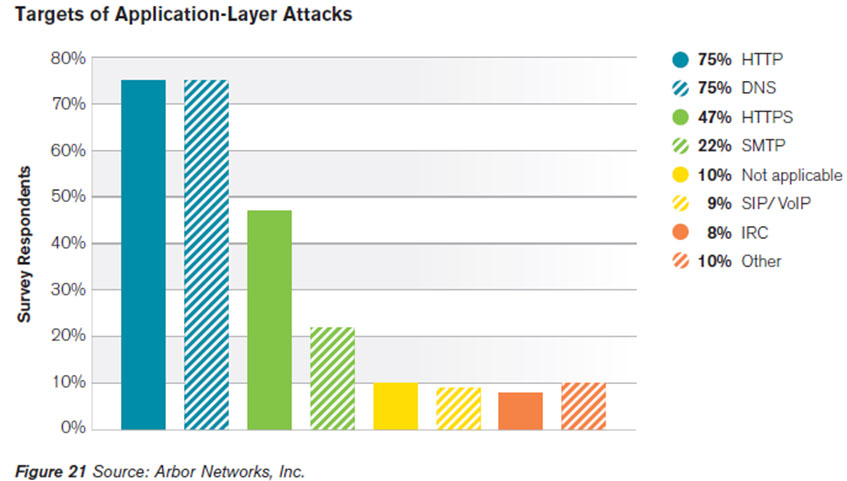
\includegraphics[width=0.35\textwidth]{fig/application-attacks-2}%
    \qquad 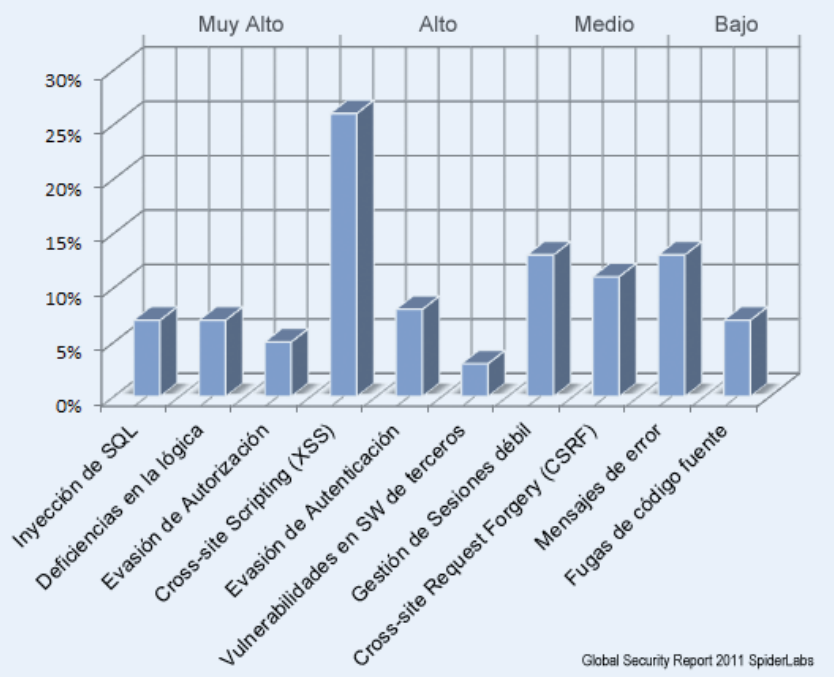
\includegraphics[width=0.35\textwidth]{fig/Vulnerabilidades_OWASP}
    \caption{\small{Ataques en capa de aplicación (fuentes Arbor \cite{articleArbor}, \acrshort{owasp} \cite{owasptop10})}}
    \label{fig:applicationattacks}
  \end{figure}
  \begin{alertblock}{Conclusión}
      Se debe realizar un esfuerzo continuo para mejor la seguridad de las plataformas web.
  \end{alertblock}
\end{frame}

\begin{frame}[shrink=20]
  \frametitle{Vulnerabilidades recientes en canales cifrados}
  Otro componente en el que se han descubierto múltiples vulnerabilidades críticas son los canales SSL/TLS.
  \begin{center}
    \rowcolors[]{1}{blue!20}{blue!5}
    \begin{tabular}{|l|l|}
      \hline
      {\bf Vulnerabilidad}   			& {\bf Componente afectado}\\
      \hline
      POODLE											&   SSL ver. 3.0        \\
      \hline
      BEAST												&   TLS ver. 1.0        \\
      \hline
      CRIME                       &   TLS compression     \\
      \hline
      BREACH                      &   HTTP compression    \\
      \hline
      Heartbleed                  &   OpenSSL ver. 1.0.1  \\
      \hline
    \end{tabular}
  \end{center}
  \begin{block}{Solución - Mitigación}
    Actualizar software y desactivar las versiones o el componente afectados.
    \par El riesgo de afectar la funcionalidad de la plataforma es bajo (dependiendo del entorno).
  \end{block}
\end{frame}

\subsection{Mecanismos de protección}
\begin{frame}[shrink]
  \frametitle{Soluciones, controles de seguridad}
  \begin{itemize}
    \item {\bf Desarrollo de código seguro}: metodologías y herramientas.
      \par Retos: Tiempo y recursos.
    \item {\bf Aplicar un ciclo de vida de aplicaciones}: Gestión de actualizaciones y configuración segura.
      \par Retos: Una actualización puede afectar al entorno, el objetivo es que la {\em aplicación funcione}.
      \par {\em chmod 777} o {\em iptables -A INPUT -j ACCEPT} funcionan.
    \item {\bf Protección perimetral de red}: Firewall de red, Sistema de Prevención de Intrusos.
      \par Reto: Visibilidad reducida.
    \item {\bf Herramientas de firewall de aplicación.}: \acrshort{waf}.
      \par Reto: Elevado coste o complejo de mantener.
  \end{itemize}
\end{frame}

\begin{frame}[shrink=20]
  \frametitle{Soluciones. Estándares y protocolos}
  Existen múltiples iniciativas cuyo objetivo es mejorar la seguridad de las aplicaciones web:
  \begin{itemize}
    \item Metodología del Ciclo de Vida de Desarrollo de Software (\acrshort{sdlc} del inglés).
    \item Estándares como el {\em Payment Card Industry Data Security Standard} (PCI DSS~\cite{pcidssrequirements}).
    \item TLS versión 1.3.
    \item HTTP/2.
    \item TLS Server Name Indication (SNI~\cite{wiki:TLSSNI}).
    \item Security Headers.
  \end{itemize}
  \begin{block}{Uso e implementación}
    Estas soluciones están disponibles y ofrecen mecanismos válidos para mejorar la seguridad de las plataformas web pero su implementación puede ser compleja.
  \end{block}
\end{frame}

\begin{frame}[shrink=10]
  \frametitle{Uso e implementación}
  Las alternativas implican un coste elevado, implementar soluciones complejas o aceptar el riesgo de seguridad. Y el resultado es el siguiente:
	\begin{columns}
	\begin{column}{0.3\textwidth}
		\begin{figure}
			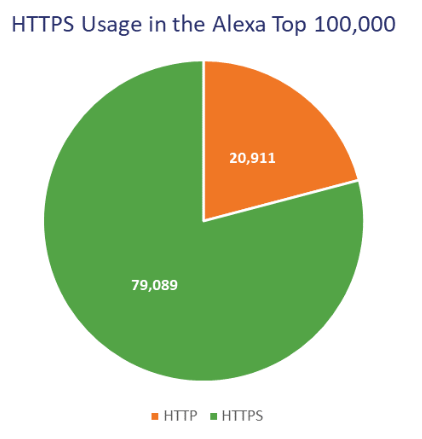
\includegraphics[width=0.9\textwidth]{fig/ImplementationHTTPHTTPS}
      \caption{\small{Tráfico HTTP versus HTTPS ~\cite{thesslstore}}}
		\end{figure}
	\end{column}
	\begin{column}{0.7\textwidth}  %%<--- here
		\begin{figure}
			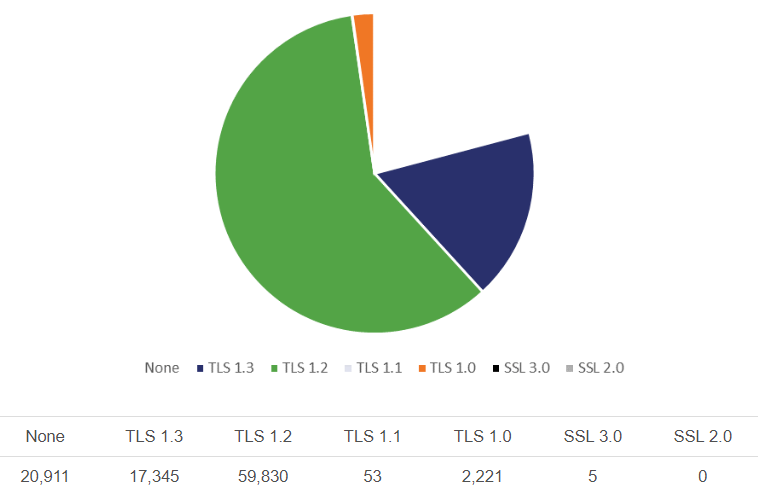
\includegraphics[width=0.7\textwidth]{fig/ImplementationSSLTLS}
      \caption{\small{Máxima versión SSL/TLS soportada~\cite{thesslstore}}}
		\end{figure}
	\end{column}
	\end{columns}
  \begin{block}{Uso e implementación}
  Se ha elegido la versión SSL/TLS como ejemplo de un vector de ataque conocido popularmente cuya mitigación es sencilla.
  \end{block}
\end{frame}

\begin{frame}[shrink=20]
  \frametitle{Visibilidad reducida}
    \begin{figure}[c]
			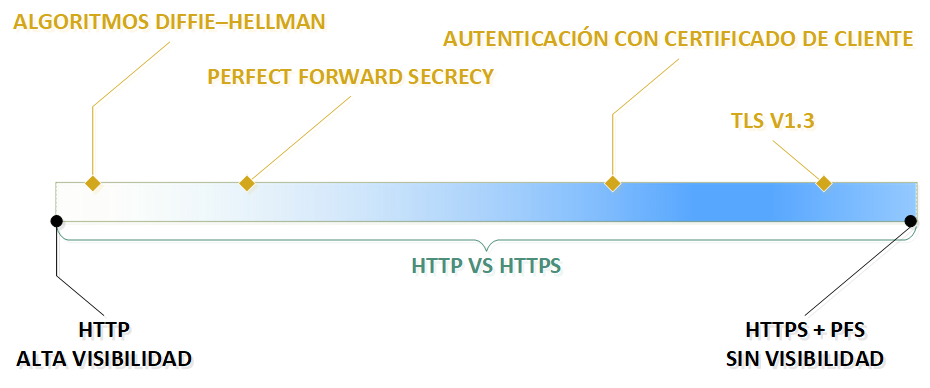
\includegraphics[width=0.9\textwidth]{fig/TLS_Visibility}
      \caption{\small{Evolución de HTTP a HTTPS con {\em Diffie–Hellman}}}
		\end{figure}
\end{frame}

\subsection{¿Qué es un WAF?}
\begin{frame}[shrink=20,fragile]
  \frametitle{\acrlong{waf} (\acrshort{waf})}
  \begin{exampleblock}{¿Qué es un WAF?}
    Un WAF es una herramienta especializada en filtrar, monitorizar y bloquear las conexiones desde y hacia una aplicación web (Fuente: Instituto Nacional de Ciberseguridad~\cite{incibewaf}).
  \end{exampleblock}
  Características principales:
  \begin{itemize}
    \item Analiza el tráfico web: Entiende GET, POST, parámetros URL, etc.
    \item Se aplican políticas y reglas de filtrado. Por ejemplo:
        \begin{lstlisting}
admin'--
' or 1=1#
' or 1=1-- -
        \end{lstlisting}
    \item Listas blancas o negras de User Agents, IP, caracteres aceptados en URL o formularios, etc.
  \end{itemize}
\end{frame}

